\documentclass[12pt]{article}
\usepackage[utf8]{inputenc}
\usepackage{amsthm}
\usepackage{amsmath}
\usepackage{amsfonts}
\usepackage{amssymb}
\usepackage{mathtools}
\usepackage{tikz}
\usepackage{graphicx}
\usepackage{caption}
\usepackage{subcaption}
\usepackage{hyperref}
\usepackage{float}
\usepackage{blindtext}
\usepackage{titlesec}
%\usepackage[legalpaper, margin=1.1in]{geometry}
\usepackage{titlesec}
%\usepackage{setspace} \doublespacing


\graphicspath{ {./graphs/} }

\title{STA 2503/MMF 1928 Project 1 - American Options}
\author{Siyu Jia, Dixin Mou, Zixun Zhai}
\date{2022/10/17}

\begin{document}
\begin{titlepage}
  \begin{center}
      \vspace*{7cm}

      \textbf{STA 2503/MMF 1928 Project 1 - American Options}

      % \vspace{0.5cm}
      %  Thesis Subtitle
           
      \vspace{1.5cm}

      \textbf{Siyu Jia, Dixin Mou, Zixun Zhai}

      \vfill
           
      % A thesis presented for the degree of\\
      % Doctor of Philosophy
           
      \vspace{0.8cm}
           
      % Department Name\\
      University of Toronto\\
      Toronto, Ontario, Canada\\
      October $18^{th}$, 2022 
           
  \end{center}
\end{titlepage}


\section{Abstract}
An American option is one of the options contracts that allows holders to exercise the option rights. Different from the European option, which can only exercise on the day of expiration, 
the American option allows holders to exercise the option at any time before and on the day of expiration, providing a chance for them to gain profit once the stock price gets better. 
This project provides the framework and valuation for the American put option using the binomial tree and Cox-Ross-Rubinstein model. The final report includes the exercises of the model 
on different time slots, profit/loss analysis, and distribution of the model parameters to build up a more comprehensive understanding of the American put option behaviors based on the CRR model. 

\newpage
\tableofcontents

\newpage
\listoffigures

\newpage
\section{Introduction}
This report focuses on the implementation and application of the binomial tree model on American put options. Compared with the Black-Scholes model, the discrete binomial tree model is more intuitive 
and often applied in a practical situations as an approximation of Black-Scholes model. The assumption of the model is that there are two outcomes with one move up and one move down with recombining features, calculating 
the asset and the option for multiple periods with results. By implementing the CRR model with the base set of parameters and additionally, considering the interest rate, this report builds up an adjusted 
CRR model to better evaluate the American put option performance.


\section{Model Setup}
Suppose that an asset price process $S = (S_{tk})_{k\in (0,1,\ldots,N)}$ (with $t_k = k\Delta t$ and $\Delta t = \frac{T}{N}$, for a fixed $N$) are given by the stochastic dynamics:
\[S_{t_k} = S_{t_{k-1}}e^{r\Delta t + \sigma \sqrt{\Delta t} \epsilon_k}\]
where $\epsilon_k$ and iid rv with $\epsilon_k \in \{+1, -1\}$ and
\[ \mathbb{P} (\epsilon_k = \pm 1) = \frac{1}{2}(1 \pm \frac{(\mu - r) - \frac{1}{2}\sigma^2}{\sigma}\sqrt{\Delta t}) \]
Here, $r\ge 0$ and $\sigma > 0$ are constants.
\\
Moreover, let $B_t = (B_{t_k})_{t\in \{ 0,1,\ldots, N \}}$ denot the back accnount with $B_t = e^{rt}$.
% \\
% \begin{tikzpicture}[level distance=30mm,sibling distance=40mm,every node/.style={fill=blue!30,circle,inner sep=5pt}]
%   \node {$S_{t_k}$}
%   child[grow=right] {
%   child {node{$S_{t_k}e^{r\Delta t-\sigma \sqrt{\Delta t}}$}} child {node{$S_{t_k}e^{r\Delta t+\sigma \sqrt{\Delta t}}$}}
%   };
% \end{tikzpicture}
% \\
% \begin{tikzpicture}[level distance=30mm,sibling distance=40mm,every node/.style={fill=blue!30,circle,inner sep=5pt}, scale = 0.9]
%   \node {$B_{t_k} = e^{rt_k}$}
%   child[grow=right] {
%   child {node{$e^{rt_{k+1}} = e^{r(t_k + \Delta t)}$}} child {node{$e^{rt_{k+1}} = e^{r(t_k + \Delta t)}$}}
%   };
% \end{tikzpicture}


\section{Methodology}
To investigate the statistical process of the price process $S$ and especially $S_T$, it is necessary to disocver to its distibution as well as the risk-neutral probability. 

\subsection{Distribution of $S_T$}
Claim that $S_T \xrightarrow[N \rightarrow \infty]{d} lognormal$ with $log(S_T/S_0) \xrightarrow[N \rightarrow \infty]{d} (\mu - \frac{1}{2}\sigma^2)T + \sigma^2 TZ$ 
where $Z \stackrel{\mathbb{P}}{\sim} \mathcal{N}(0, 1)$. The following is the proof.\\

\begin{proof}
Let $X^(N)$ denote the random variable $X^{(N)} := log(S_T/S_0)$.
\\\\
Consider \[X^{(N)} = \log(\frac{S_T}{S_0}) = \sum_{n=1}^N (r\Delta t+\sigma \sqrt[]{\Delta t} \epsilon_n)\]
The m.g.f of $X^{(N)}$ is: \\
\begin{align*}
  \mathbb{E}^\mathbb{P}[e^{u X^{(N)}}] & =  \mathbb{E}^\mathbb{P}[e^{\sum_{n=1}^N (u r\Delta t+u\sigma \sqrt[]{\Delta t} \epsilon_n)}] \\
  & = \mathbb{E}^\mathbb{P} [\prod_{n=1}^N e^{u r\Delta t+u\sigma \sqrt[]{\Delta t} \epsilon_n}] \\
  & = (\mathbb{E}^\mathbb{P} [e^{u r\Delta t+u\sigma \sqrt[]{\Delta t} \epsilon_1}])^N \tag*{as $\epsilon_n$ is i.i.d}
\end{align*}
Investigate the inner term $\mathbb{E}^\mathbb{P} [e^{u r\Delta t+ u\sigma \sqrt[]{\Delta t} \epsilon_1}]$:
\begin{align*}
  \mathbb{E}^\mathbb{P} [e^{u r\Delta t+u\sigma \sqrt{\Delta t} \epsilon_1}] &= e^{u r\Delta t +u\sigma \sqrt{\Delta t}} \cdot \frac{1}{2} (1 + \frac{(\mu -r) - \frac{1}{2}\sigma^2}{\sigma} \sqrt{\Delta t}) \\ 
    & \quad + e^{u r\Delta t-u\sigma \sqrt[]{\Delta t}} \cdot \frac{1}{2} (1 - \frac{(\mu -r) - \frac{1}{2}\sigma^2}{\sigma} \sqrt{\Delta t}) \\
    &= [1+u r\Delta t+u \sigma \sqrt{\Delta t} +\frac{1}{2}u^2\sigma^2\Delta t + o(\Delta t)] \cdot \frac{1}{2} (1 + \frac{(\mu -r) - \frac{1}{2}\sigma^2}{\sigma} \sqrt{\Delta t}) \\ 
    & \quad + [1+u r\Delta t-u \sigma \sqrt{\Delta t} +\frac{1}{2}u^2\sigma^2\Delta t + o(\Delta t)] \cdot \frac{1}{2} (1 - \frac{(\mu -r) - \frac{1}{2}\sigma^2}{\sigma} \sqrt{\Delta t}) 
\end{align*} \\
\\
Note all terms containing $\Delta t$ with order 2 or higher are collected in $o(\Delta t)$ because as $N\rightarrow \infty$ 
and $\Delta t \rightarrow 0$, $o(\Delta t)$ will converge to 0 faster than $\Delta t$ or $\Delta t$ with lower orders.
And later $o(\sqrt{\Delta t})$ is defined in a similar manner. 
\\ \\ 
Continue the algebra manipulation:
\begin{align*}
  \mathbb{E}^\mathbb{P} [e^{u r\Delta t+u\sigma \sqrt{\Delta t} \epsilon_n}] &= [1+u r\Delta t+u \sigma \sqrt{\Delta t} +\frac{1}{2}u^2\sigma^2\Delta t + o(\Delta t)] \cdot \frac{1}{2} (1 + \frac{(\mu -r) - \frac{1}{2}\sigma^2}{\sigma} \sqrt{\Delta t}) \\ 
    & \quad + [1+u r\Delta t-u \sigma \sqrt{\Delta t} +\frac{1}{2}u^2\sigma^2\Delta t + o(\Delta t)] \cdot \frac{1}{2} (1 - \frac{(\mu -r) - \frac{1}{2}\sigma^2}{\sigma} \sqrt{\Delta t}) \\
    &= \frac{1}{2}[ 1 + \frac{(\mu - r) - \frac{1}{2}\sigma^2}{\sigma}\sqrt{\Delta t} + u r \Delta t + u \sigma \sqrt{\Delta t} \\
    & \quad + u((\mu -r) - \frac{1}{2}\sigma^2)\Delta t + \frac{1}{2}u^2 \sigma^2 \Delta t \\
    & \quad + 1 - \frac{(\mu - r) - \frac{1}{2}\sigma^2}{\sigma}\sqrt{\Delta t} + ur \Delta t - u\sigma \sqrt{\Delta t} \\
    & \quad + u((\mu -r) - \frac{1}{2}\sigma^2)\Delta t + \frac{1}{2}u^2 \sigma^2 \Delta t + o(\Delta t)] \\
    &= 1 + ur \Delta t + u((\mu - r) - \frac{1}{2}\sigma^2)\Delta t + \frac{1}{2}u^2 \sigma^2 \Delta t + o(\Delta t) \\
    &= 1 + (ur + u\mu - ur -\frac{1}{2}u \sigma^2 + \frac{1}{2}u^2 \sigma^2)\Delta t + o(\Delta t) \\
    &= 1 + (u (\mu - \frac{1}{2}\sigma^2) + \frac{1}{2}u^2 \sigma^2)\Delta t + o(\Delta t)\\
    &= e^{(u (\mu - \frac{1}{2}\sigma^2) + \frac{1}{2}u^2 \sigma^2)\Delta t} + o(\Delta t)
\end{align*} 
As a result:
\begin{align*}
  \mathbb{E}^\mathbb{P}[e^{u X^{(N)}}] & = (e^{(u (\mu - \frac{1}{2}\sigma^2) + \frac{1}{2}u^2 \sigma^2)\Delta t} + o(\Delta t))^N\\
    &=  e^{(u(\mu - \frac{1}{2}\sigma^2)T + \frac{1}{2}u^2 \sigma^2T)} \tag*{as $N \rightarrow \infty$ and $\Delta t = \frac{T}{N}$}
\end{align*}
\\
Notice that the m.g.f of the $X^{(N)}$ is equal to the m.g.f of a random variable $Y$ whcih follows the normal distribution with mean $(\mu - \frac{1}{2}\sigma^2)T$ and
variance $\sigma^2 T$.
\\ \\
Thus,
\[X^{(N)} \xrightarrow[N \rightarrow \infty]{d} (\mu - \frac{1}{2}\sigma^2)T + \sigma^2 TZ\]
where 
\[Z \stackrel{\mathbb{P}}{\sim} \mathcal{N}(0, 1)\] 
\end{proof}



\subsection{Risk-neutral Probability $\mathbb{Q}$ and $\mathbb{Q}^S$}
Another interesting quetison is what the risk-neutral probability is with repect to the price process $S$ and $B$ as the numeraire asset. And how these properties change when using
$S$ as the numeraire asset. 

\subsubsection{$\mathbb{Q}$-Probability}
Let $\mathbb{Q}$ refer to the martingale measure induced by using the asset $B$ as the numeraire. Define $\mathbb{Q}(\epsilon_k = \pm 1)$ where $\mathbb{Q}(\epsilon_k =1) = q_k$ and $\mathbb{Q}(\epsilon_k =-1) = 1-q_k$. Consider 
time $t_k$ and $t_{k+1}$. \\ \\ 
Construct the following $\mathbb{Q}$-martingale:
\begin{align*}
&\qquad \frac{S_{t_k}}{e^{rt_k}} = q_k\frac{S_{t_k}e^{r\Delta t + \sigma \sqrt{\Delta t}}}{e^{r(t_k+\Delta t)}} + (1-q_k)\frac{S_{t_k}e^{r\Delta t - \sigma \sqrt{\Delta t}}}{e^{r(t_k+\Delta t)}}\\
&\Rightarrow 1 = q_k\frac{e^{r\Delta t + \sigma \sqrt{\Delta t}}}{e^{r\Delta t}} + (1-q_k) \frac{e^{r\Delta t - \sigma \sqrt{\Delta t}}}{e^{r\Delta t}} \\
&\Rightarrow q_k(e^{r\Delta t + \sigma \sqrt{\Delta t}} - e^{r\Delta t - \sigma \sqrt{\Delta t}}) = e^{r\Delta t} - e^{r\Delta t - \sigma \sqrt{\Delta t}} \\
&\Rightarrow q := q_k = q = \frac{e^{r\Delta t} - e^{r\Delta t - \sigma \sqrt{\Delta t}}}{e^{r\Delta t + \sigma \sqrt{\Delta t}} - e^{r\Delta t - \sigma \sqrt{\Delta t}}} \tag*{As $q_k$ does not depend on $k$} \\
& \Rightarrow q = \frac{1-e^{ - \sigma \sqrt{\Delta t}}}{e^{  \sigma \sqrt{\Delta t}}-e^{ - \sigma \sqrt{\Delta t}}}
\end{align*} 
\\\\
Taylor-expand exponential terms and collect all terms containing $\Delta t$ with order 2 or higher to be $o(\Delta t)$:
\begin{align*}
  q &= \frac{1-e^{ - \sigma \sqrt{\Delta t}}}{e^{  \sigma \sqrt{\Delta t}}-e^{ - \sigma \sqrt{\Delta t}}}\\
  &= \frac{1-(1 - \sigma \sqrt{\Delta t} + \frac{1}{2}\sigma^2\Delta t) + o(\Delta t)}
    {1 + \sigma \sqrt{\Delta t} + \frac{1}{2}\sigma^2\Delta t^2 - (1 - \sigma \sqrt{\Delta t} + \frac{1}{2}\sigma^2\Delta t^2) + o(\Delta t)} \\
  &= \frac{\sigma \sqrt{\Delta t} - \frac{1}{2} \sigma^2\Delta t + o(\Delta t)}{2\sigma\sqrt{\Delta t} + o(\Delta t)}\\
  &= \frac{1}{2} - \frac{1}{4}\sigma\sqrt{\Delta t} + o(\sqrt{\Delta t}) \\
  &= \frac{1}{2}(1 - \frac{1}{2}\sigma\sqrt{\Delta t}) + o(\sqrt{\Delta t})
\end{align*}

\subsubsection{$S_T$ Distribution Regarding $\mathbb{Q}$}
This section derives the $\mathbb{Q}$ distribution of $S_T$ as $N \rightarrow \infty$. Define $X_T = log(\frac{S_T}{S_0})$, then: 
\[X_T = \log(\frac{S_T}{S_0}) = \log(e^{\sum_{n=1}^N r\Delta t + \sigma \sqrt{\Delta t} \epsilon_n}) = \sum_{n=1}^N r\Delta t + \sigma \sqrt{\Delta t} \epsilon_n \]
Consider the m.g.f of $X_T$:
\begin{align*}
  \mathbb{E}^\mathbb{P}[e^{u X_T}] & =  \mathbb{E}^\mathbb{P}[e^{\sum_{n=1}^N (u r\Delta t+u\sigma \sqrt[]{\Delta t} \epsilon_n)}] \\
  & = \mathbb{E}^\mathbb{P} [\prod_{n=1}^N e^{u r\Delta t+u\sigma \sqrt[]{\Delta t} \epsilon_n}] \\
  & = (\mathbb{E}^\mathbb{P} [e^{u r\Delta t+u\sigma \sqrt[]{\Delta t} \epsilon_1}])^N \tag*{as $\epsilon_n$ is i.i.d}
\end{align*}
Investigate the inner term $\mathbb{E}^\mathbb{P} [e^{u r\Delta t+ u\sigma \sqrt[]{\Delta t} \epsilon_1}]$:
\begin{align*}
  \mathbb{E}^\mathbb{P} [e^{u r\Delta t+u\sigma \sqrt{\Delta t} \epsilon_1}] &= e^{u r\Delta t +u\sigma \sqrt{\Delta t}} \cdot \frac{1}{2} (1 - \frac{1}{2}{\sigma} \sqrt{\Delta t} + o(\sqrt{\Delta t})) \\ 
    & \quad + e^{u r\Delta t-u\sigma \sqrt[]{\Delta t}} \cdot \frac{1}{2} (1 + \frac{1}{2}{\sigma} \sqrt{\Delta t} + o(\sqrt{\Delta t})) \\
    &= [1+u r\Delta t+u \sigma \sqrt{\Delta t} +\frac{1}{2}u^2\sigma^2\Delta t + o(\Delta t)] \cdot \frac{1}{2} (1 - \frac{1}{2}{\sigma} \sqrt{\Delta t} + o(\sqrt{\Delta t})) \\ 
    & \quad + [1+u r\Delta t-u \sigma \sqrt{\Delta t} +\frac{1}{2}u^2\sigma^2\Delta t + o(\Delta t)] \cdot \frac{1}{2} (1 + \frac{1}{2}{\sigma} \sqrt{\Delta t} + o(\sqrt{\Delta t})) \\
    &= \frac{1}{2}[1 - \frac{1}{2}\sigma\sqrt{\Delta t} + ur\Delta t + u\sigma \sqrt{\Delta t} - \frac{1}{2}u\sigma^2\Delta t + \frac{1}{2}u^2\sigma^2\Delta t \\
    & \quad + 1 + \frac{1}{2}\sigma\sqrt{\Delta t} + ur\Delta t - u\sigma \sqrt{\Delta t} - \frac{1}{2}u\sigma^2\Delta t + \frac{1}{2}u^2\sigma^2\Delta t + o(\Delta t)] \\
    &= 1 + ur\Delta t - \frac{1}{2} u\sigma^2\Delta t + \frac{1}{2}u^2\sigma^2\Delta t + o(\Delta t) \\
    &= 1 + (u(r-\frac{1}{2}\sigma^2) + \frac{1}{2}u^2\sigma^2) \Delta t + o(\Delta t) \\
    &= e^{(u(r-\frac{1}{2}\sigma^2) + \frac{1}{2}u^2\sigma^2) \Delta t + o(\Delta t)}
\end{align*}
As a result, the m.g.f of $X_T$ to be:
\begin{align*}
  \mathbb{E}^\mathbb{P}[e^{u X_T}] &= (\mathbb{E}^\mathbb{P} [e^{u r\Delta t+u\sigma \sqrt[]{\Delta t} \epsilon_1}])^N \\
  &= (e^{(u(r-\frac{1}{2}\sigma^2) + \frac{1}{2}u^2\sigma^2) \Delta t + o(\Delta t)})^N\\
  &= e^{(u(r - \frac{1}{2}\sigma^2)T + \frac{1}{2}u^2 \sigma^2T)} \tag*{as $N \rightarrow \infty$ and $\Delta t = \frac{T}{N}$}
\end{align*}
\\
Notice that the m.g.f of the $X_T$ is equal to the m.g.f of a random variable $Y$ whcih follows the normal distribution with mean $(r - \frac{1}{2}\sigma^2)T$ and
variance $\sigma^2 T$. Thus, as $S_T  \xrightarrow[N \rightarrow \infty]{d, \mathbb{Q}} lognormal$.\\
Specifically: 
\[ log(\frac{S_T}{S_0})  \xrightarrow[N \rightarrow \infty]{d, \mathbb{Q}} N((r - \frac{1}{2}\sigma^2)T,\sigma^2 T) \]


\subsubsection{$\mathbb{Q}^S$-Probability}
Conduct a similar analysis using $S$ as the numeraire asset. Let $\mathbb{Q}^S$ refer to the martingale measure induced by using the asset $S$ as the numeraire.
Define $\mathbb{Q}^S(\epsilon_k = \pm 1)$ where $\mathbb{Q}^S(\epsilon_k =1) = h_k$ and $\mathbb{Q}^S(\epsilon_k =-1) = 1-h_k$.\\ \\
Construct the following $\mathbb{Q}^S$-martingale:
\begin{align*}
  &\qquad \frac{e^{rt_k}}{S_{t_k}} = h_k\frac{e^{r(t_k+\Delta t)}}{S_{t_k}e^{r\Delta t + \sigma \sqrt{\Delta t}}} + (1-h_k)\frac{e^{r(t_k+\Delta t)}}{S_{t_k}e^{r\Delta t - \sigma \sqrt{\Delta t}}}\\
  &\Rightarrow  1 = h_k\frac{e^{r\Delta t}}{e^{r\Delta t + \sigma \sqrt{\Delta t}}} + (1-h_k) \frac{e^{r\Delta t}}{e^{r\Delta t - \sigma \sqrt{\Delta t}}} \\
  &\Rightarrow e^{2r\Delta t} = h_ke^{2r\Delta t - \sigma \sqrt{\Delta t}} + (1-h_k)e^{2r\Delta t + \sigma \sqrt{\Delta t}}\\
  &\Rightarrow e^{2r\Delta t} - e^{2r\Delta t + \sigma \sqrt{\Delta t}} = h_k(e^{2r\Delta t - \sigma \sqrt{\Delta t}} - e^{2r\Delta t + \sigma \sqrt{\Delta t}}) \\
  &\Rightarrow h:= h_k = \frac{e^{2r\Delta t} - e^{2r\Delta t + \sigma \sqrt{\Delta t}}}{e^{2r\Delta t - \sigma \sqrt{\Delta t}} - e^{2r\Delta t + \sigma \sqrt{\Delta t}}} \tag*{As $h_k$ does not depend on $k$} \\
  & \Rightarrow h = \frac{1-e^{\sigma \sqrt{\Delta t}}}{e^{-\sigma \sqrt{\Delta t}}-e^{\sigma \sqrt{\Delta t}}}
\end{align*}
Taylor-expand exponential terms and collect all terms containing $\Delta t$ with order 2 or higher to be $o(\Delta t)$:
\begin{align*}
  h &= \frac{1-e^{\sigma \sqrt{\Delta t}}}{e^{-\sigma \sqrt{\Delta t}}-e^{\sigma \sqrt{\Delta t}}} \\
    &=\frac{1-(1 + \sigma \sqrt{\Delta t} + \frac{1}{2}\sigma^2\Delta t) + o(\Delta t)}
      {1 - \sigma \sqrt{\Delta t} + \frac{1}{2}\sigma^2\Delta t^2 - (1 + \sigma \sqrt{\Delta t} + \frac{1}{2}\sigma^2\Delta t^2) + o(\Delta t)} \\
    &= \frac{\sigma \sqrt{\Delta t} + \frac{1}{2} \sigma^2\Delta t + o(\Delta t)}{2\sigma\sqrt{\Delta t} + o(\Delta t)}\\
    &= \frac{1}{2} + \frac{1}{4}\sigma\sqrt{\Delta t} + o(\sqrt{\Delta t}) \\
    &= \frac{1}{2}(1 + \frac{1}{2}\sigma\sqrt{\Delta t}) + o(\sqrt{\Delta t})
\end{align*}


\subsubsection{$S_T$ Distribution Regarding $\mathbb{Q}^S$}
This section derives the $\mathbb{Q}^S$ distribution of $S_T$ as $N \rightarrow \infty$.Firstly, define $X_T = log(\frac{S_T}{S_0})$, then: 
\[X_T = \log(\frac{S_T}{S_0}) = \log(e^{\sum_{n=1}^N r\Delta t + \sigma \sqrt{\Delta t} \epsilon_n}) = \sum_{n=1}^N r\Delta t + \sigma \sqrt{\Delta t} \epsilon_n \]
Consider the m.g.f of $X_T$:
\begin{align*}
  \mathbb{E}^\mathbb{P}[e^{u X_T}] & =  \mathbb{E}^\mathbb{P}[e^{\sum_{n=1}^N (u r\Delta t+u\sigma \sqrt[]{\Delta t} \epsilon_n)}] \\
  & = \mathbb{E}^\mathbb{P} [\prod_{n=1}^N e^{u r\Delta t+u\sigma \sqrt[]{\Delta t} \epsilon_n}] \\
  & = (\mathbb{E}^\mathbb{P} [e^{u r\Delta t+u\sigma \sqrt[]{\Delta t} \epsilon_1}])^N \tag*{as $\epsilon_n$ is i.i.d}
\end{align*}
Investigate the inner term $\mathbb{E}^\mathbb{P} [e^{u r\Delta t+ u\sigma \sqrt[]{\Delta t} \epsilon_1}]$:
\begin{align*}
  \mathbb{E}^\mathbb{P} [e^{u r\Delta t+u\sigma \sqrt{\Delta t} \epsilon_1}] &= e^{u r\Delta t +u\sigma \sqrt{\Delta t}} \cdot \frac{1}{2} (1 + \frac{1}{2}{\sigma} \sqrt{\Delta t} + o(\sqrt{\Delta t})) \\ 
    & \quad + e^{u r\Delta t-u\sigma \sqrt[]{\Delta t}} \cdot \frac{1}{2} (1 - \frac{1}{2}{\sigma} \sqrt{\Delta t} + o(\sqrt{\Delta t})) \\
    &= [1+u r\Delta t+u \sigma \sqrt{\Delta t} +\frac{1}{2}u^2\sigma^2\Delta t + o(\Delta t)] \cdot \frac{1}{2} (1 + \frac{1}{2}{\sigma} \sqrt{\Delta t} + o(\sqrt{\Delta t})) \\ 
    & \quad + [1+u r\Delta t-u \sigma \sqrt{\Delta t} +\frac{1}{2}u^2\sigma^2\Delta t + o(\Delta t)] \cdot \frac{1}{2} (1 - \frac{1}{2}{\sigma} \sqrt{\Delta t} + o(\sqrt{\Delta t})) \\
    &= \frac{1}{2}[1 + \frac{1}{2}\sigma\sqrt{\Delta t} + ur\Delta t + u\sigma \sqrt{\Delta t} + \frac{1}{2}u\sigma^2\Delta t + \frac{1}{2}u^2\sigma^2\Delta t \\
    & \quad + 1 - \frac{1}{2}\sigma\sqrt{\Delta t} + ur\Delta t - u\sigma \sqrt{\Delta t} + \frac{1}{2}u\sigma^2\Delta t + \frac{1}{2}u^2\sigma^2\Delta t + o(\Delta t)] \\
    &= 1 + ur\Delta t + \frac{1}{2} u\sigma^2\Delta t + \frac{1}{2}u^2\sigma^2\Delta t + o(\Delta t) \\
    &= 1 + (u(r+\frac{1}{2}\sigma^2) + \frac{1}{2}u^2\sigma^2) \Delta t + o(\Delta t) \\
    &= e^{(u(r+\frac{1}{2}\sigma^2) + \frac{1}{2}u^2\sigma^2) \Delta t + o(\Delta t)}
\end{align*}
Then the m.g.f of $X_T$ is:
\begin{align*}
  \mathbb{E}^\mathbb{P}[e^{u X_T}] &= (\mathbb{E}^\mathbb{P} [e^{u r\Delta t+u\sigma \sqrt[]{\Delta t} \epsilon_1}])^N \\
  &= (e^{(u(r+\frac{1}{2}\sigma^2) + \frac{1}{2}u^2\sigma^2) \Delta t + o(\Delta t)})^N\\
  &= e^{(u(r + \frac{1}{2}\sigma^2)T + \frac{1}{2}u^2 \sigma^2T)} \tag*{as $N \rightarrow \infty$ and $\Delta t = \frac{T}{N}$}
\end{align*}
\\
Notice that the m.g.f of the $X_T$ is equal to the m.g.f of a random variable $Y$ whcih follows the normal distribution with mean $(r + \frac{1}{2}\sigma^2)T$ and
variance $\sigma^2 T$. Thus, as $S_T  \xrightarrow[N \rightarrow \infty]{d, \mathbb{Q}^S} lognormal$.\\
Specifically: 
\[ log(\frac{S_T}{S_0})  \xrightarrow[N \rightarrow \infty]{d, \mathbb{Q}^S} N((r + \frac{1}{2}\sigma^2)T,\sigma^2 T) \]


\section{Result}
This part contains an evaluation of an American option put option based on the model specified in model setup section with the 
following parameters.
$$ T = 1, S_0 =10, \mu = 0.05, \sigma = 0.2, r=0.02, N = 5000$$

\subsection{Early Exercise Boundary}
The early exercise boundary is defined as a set of underlying asset prices with respect to the minimum possible values of the option. 
The exercising time at each time step is the minimum of possible values of the American option given the condition that the corresponding 
payoff is greater and equal to its corresponding intrinsic value. 
\\\\
The exercise boundary computed under the binomial tree model follows an increasing, concave curve as time closes to maturity time.  \\
\begin{figure}[H]
  \centering
  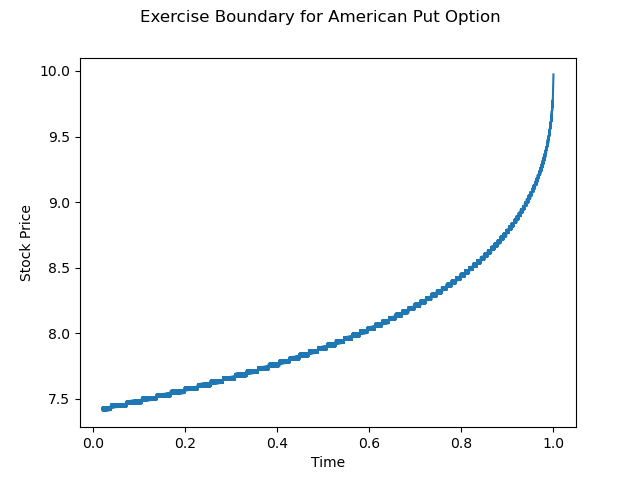
\includegraphics[scale=0.5]{3a-i.png}
  \caption[Exercise Boundary for American Put]{Exercise Boundary for American Put}
\end{figure}


\subsection{Hedging Strategy}
It is more convenient to analyze the stock price in the American put option and European put option by data visualizing the $\alpha$ and 
$\beta$ hedging strategy. That is, there is a self-financing portfolio $(\alpha_{t_k}, \beta_{t_k}, -1)_{k\in 0,1,\ldots, N}$, such that
\[ \alpha_{t_k}S_{t_k} + \beta_{t_k}B_{t_k} - \text{value of option at }t_k=0\]
Note: In theorem, there is no upper limit for price of the underlying asset $S$. However, the position of a hedging portfolio
converges as the stock price goes above certain point. As a result, for this analysis and analysis in the following section, figures 
with x-axis being the price range of the underlying asset are limited in the range $[0,25]$.

\begin{figure}[H]
  \centering
  \begin{subfigure}{.5\textwidth}
    \centering
    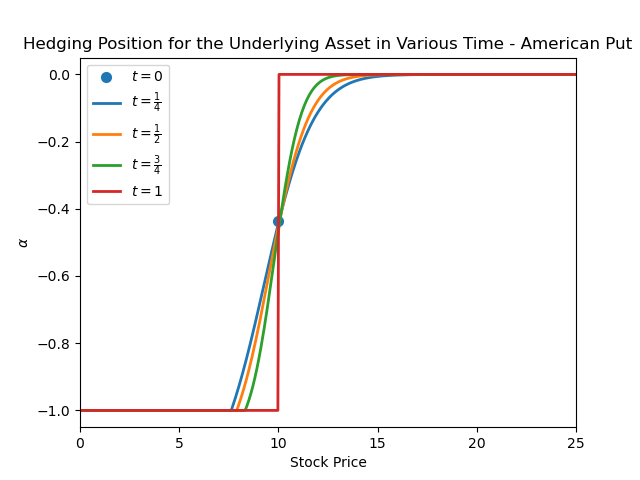
\includegraphics[width=\linewidth]{3a-ii-ap-alpha.png}
  \end{subfigure}%
  \begin{subfigure}{.5\textwidth}
    \centering
    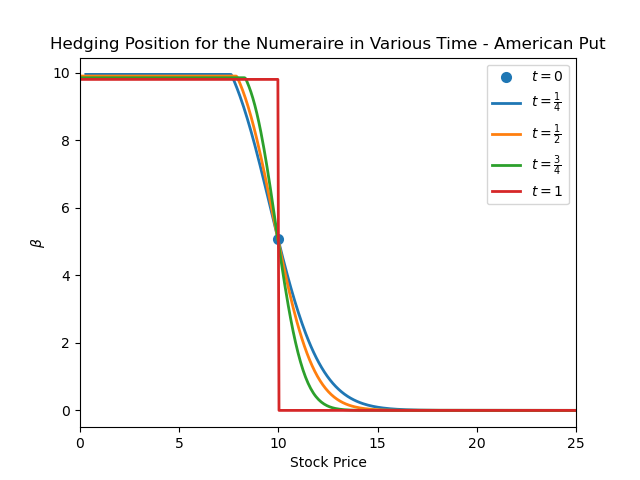
\includegraphics[width=\linewidth]{3a-ii-ap-beta.png}
    % \caption{A subfigure}
    % \label{fig:sub2}
  \end{subfigure}%
  %\caption{A figure with two subfigures}
  %\label{fig:test}

  \centering
  \begin{subfigure}{.5\textwidth}
    \centering
    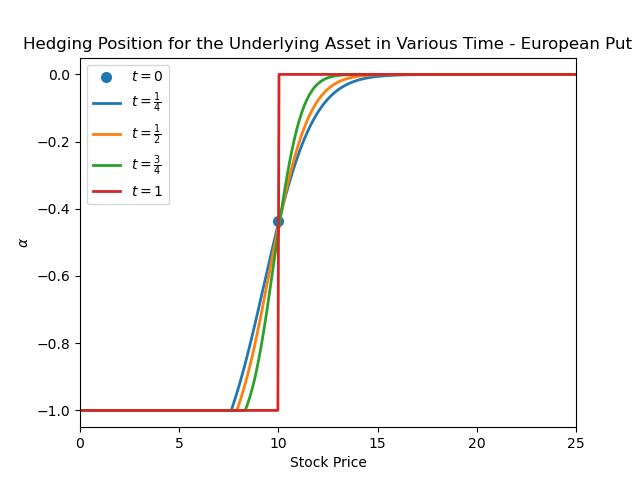
\includegraphics[width=\linewidth]{3a-ii-ep-alpha.png}
  \end{subfigure}%
  \begin{subfigure}{.5\textwidth}
    \centering
    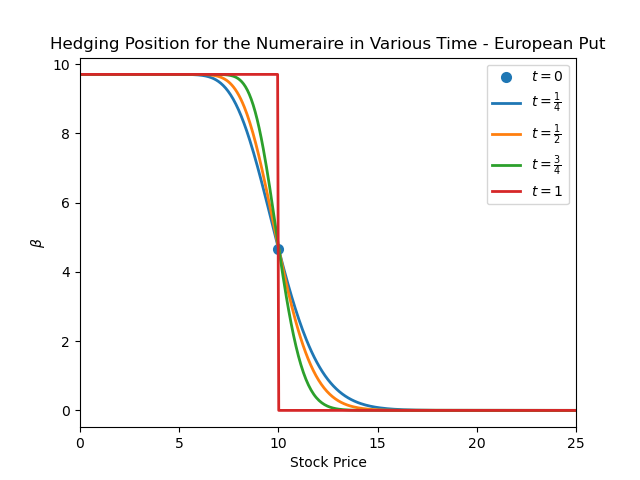
\includegraphics[width=\linewidth]{3a-ii-ep-beta.png}
  \end{subfigure}%
  \caption[Hedging Position for American/European Put Option in Various Time]{Hedging Position for American/European Put Option in Various Time}
\end{figure}

\noindent 
According to the graphs above, both the American and European put options have upward trends in the $\alpha$ hedging strategy and 
downward trends in the $\beta$ hedging strategy. When the stock price is too high,
the put option will never be exercised and of zero value. Thus there is no need to hedge, which is equavalent to say $\alpha_t = 0$ and
$\beta_t = 0$. On the other hand, when stock price goes to 0, that means the option is deep in the money and the hedge is to short a 
stock, which is equavalent to have $\alpha_t=-1$ and $\beta$ approaches $Ke^{-rt}$ where $K$ is the strike.
\\\\
Note that when $t=0$, the stock price is a known and unique value $S_0$, and hence 
there is a unique $(\alpha_0, \beta_0)$ combination for $S_0$. At the expiry $t=1$, the hedge is either to hold the stock or not as 
that is what put option holders would pay, and hence the portfolio line at $t=1$ represents this binary decision. Another interesting 
observation is that as $t$ approaches expiry, the graph tends to approach the vertical line $S_t = K$ where $K$ is the strike price. 
This makes sense as time approaches expiry, there is less decision space for changing postions.
\\\\
The difference between American options and European options is the slope of the graph. In the European put option, the slop is 
smoother, while the lines in the American put option have a non-differentiable turning point when $\alpha$ position changes from 0. 
A similar non-differentiable turning point is also witnessed in the $\beta$ hedging graph. By discussing the difference between the 
American put option and the European put option, it tends to be clear that this may result from the time for early exercise. 
The European put option can only exercise at expiration, but the American put option can exercise before the expiration. As a result, the slope in 
the American put option graph may have direct turning points, which also cause a higher risk and value.\\

\subsection{Sensitivity Analysis}
Sensitivity analysis is a process that helps determine the effect of one independent variable on another dependent variable. Normally the sensitivity 
analysis is considered when there are boundaries depending on input variables. In this section, the analysis focuses on the sensitivity of volatility 
and risk-free rate connected to stock price under both $\alpha$ and $\beta$ hedging strategies\\\\
In terms of analyzing the effect of volatility and risk-free rate on stock price, the testing model keeps a fixed in time with changes on other variables. 
When time points $t=0.25$, keep volatility and risk-free rate intervals from 0.1 to 0.5 to see the trends of changes.

\subsubsection{Volatility}
\begin{figure}[H]
  \centering
  \begin{subfigure}{.5\textwidth}
    \centering
    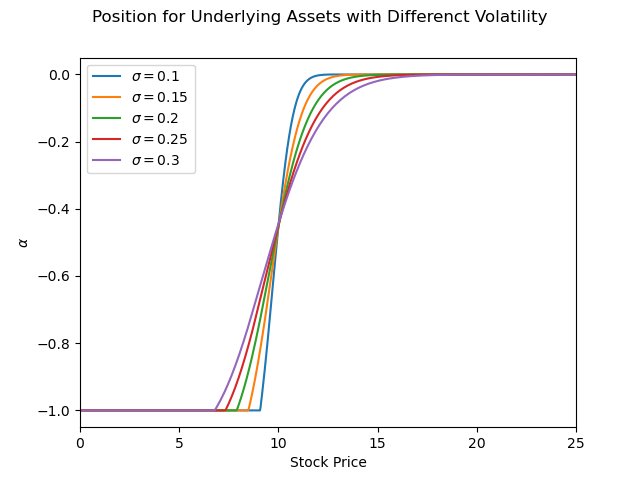
\includegraphics[width=\linewidth]{3a-iii-sigma-alpha.png}
  \end{subfigure}%
  \begin{subfigure}{.5\textwidth}
    \centering
    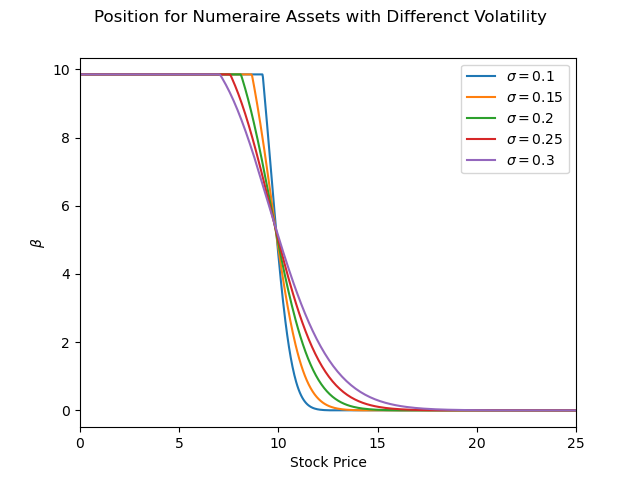
\includegraphics[width=\linewidth]{3a-iii-sigma-beta.png}
  \end{subfigure}%
  \caption[Hedging Position with Different Volatility]{Hedging Position with Different Volatility}
\end{figure}
According to the plots above, when volatility goes higher, the curve of $\alpha$ hedging becomes flatter. The relation between stock price and alpha is more sensitive, 
easily having a better return compared with the market. Similar to $\alpha$ hedging, when volatility goes higher, the curve of $\beta$ hedging becomes flatter. At this time, 
the relation between $\beta$ and stock price tends to become more elastic. 
\\\\
The financial explanation is that when volatility $\sigma$ increases, the prices of all put options on that underlying asset tend to rise. This is because the chances 
of all options finishing in the money likewise increase. So the option are more likely to have value which is necessary to hedge. Since as volatility $\sigma$ increases,
the broader the hedging range is, which means hedging position should be build for a wider range of stock price.  

\subsubsection{Risk-free Rate}
\begin{figure}[H]
  \centering
  \begin{subfigure}{.5\textwidth}
    \centering
    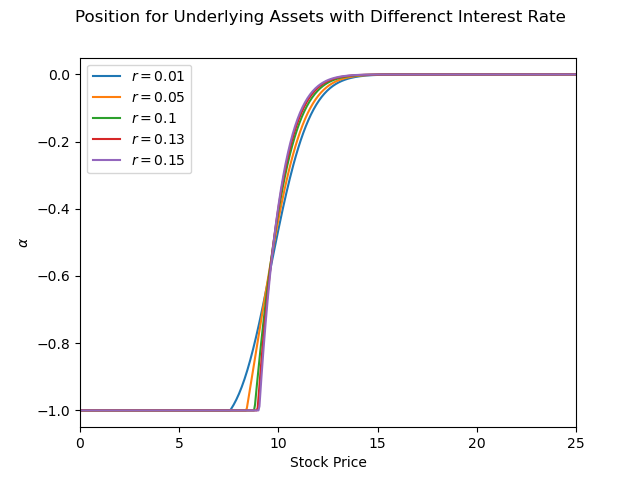
\includegraphics[width=\linewidth]{3a-iii-r-alpha.png}
  \end{subfigure}%
  \begin{subfigure}{.5\textwidth}
    \centering
    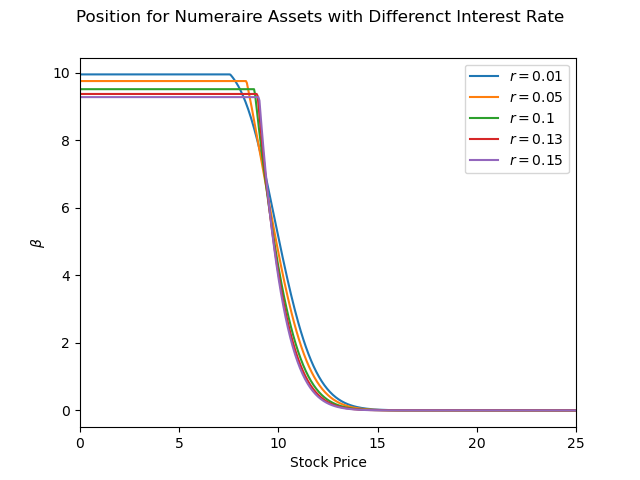
\includegraphics[width=\linewidth]{3a-iii-r-beta.png}
  \end{subfigure}%
  \caption[Hedging Position with Different Risk-free Rate]{Hedging Position with Different Risk-free Rate}
\end{figure}
When the risk-free rate goes higher, the curve of $\alpha$ hedging becomes steeper. The relation between stock price and alpha is less sensitive, harder to have the same return 
compared with the past. In $\beta$ hedging, the curve becomes steeper coming with a more inelastic relationship between $\beta$ and stock price. In this case, the rising risk-free 
rate may cause a higher standard from investors to the assets.
\\\\
The financial explanation is similar to the section above. When risk-free rate $r$ increases, the prices of all asset tend to rise. Thus, the chances 
of all options finishing in the money likewise decrease. So the option are less likely to have value which is necessary to hedge. Since as volatility $r$ increase,
the narrower the hedging range is, which means hedging position should be build for a less wide range of stock price.  

\subsubsection{Exercise Boundary Regarding Volatility and Risk-free Rate}
This section analyzes and evaluates the sensitivity of early exercise boundaries (EEB) to the change in the interest rate and volatility. The plots below take on a range of 0.1 
to 0.3 for volatility and a range of 0.01 to 0.05 for interest rate. \\\\
It is evident that the patterns of early exercise boundary for volatility and interest rate witness distinct trends. To be specific, the early exercise boundary sees a broader 
range of exercising prices over the life of the option as the increase of volatility. In contrast, the early exercise boundary experienced a narrower range of exercising prices as 
the increase of interest rate. In other words, the exercising price has a negative relationship with volatility and a positive relationship with interest rate. Worth noting that the 
amount of EEB change remains almost constant given the constant rise in volatility compared to the change of EEB becomes less and less in the condition of the constant increase in interest rates.
\\\\
These trends may relate to the larger volatility contributing to a wider stock distribution range, indicating that more nodes will become deep in the money over the option time. More occurrences of 
lower stock prices thus lead to a lower exercise boundary. Similarly, a more significant value in interest rate results in a positive impact on the probability that stock prices will go up. It then 
forms a more upper-ward binomial tree model where each node tends to be greater than the lower interest rate nodes. Therefore, this would cause a more significant value in exercise price and a higher 
exercise boundary as interest rates rise.

\begin{figure}[H]
  \centering
  \begin{subfigure}{.5\textwidth}
    \centering
    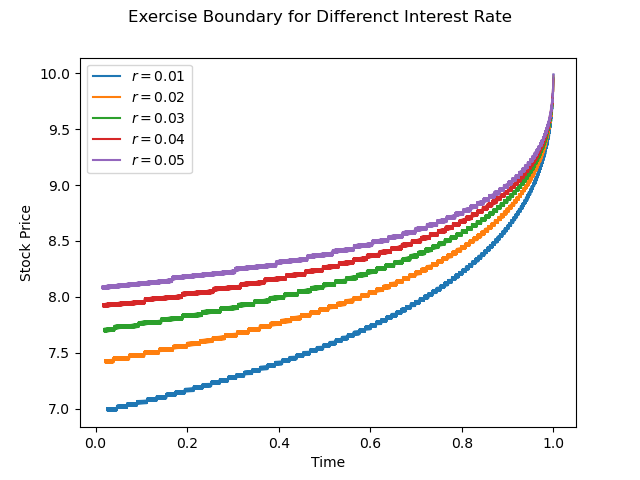
\includegraphics[width=\linewidth]{3a-iii-boundary-r.png}
  \end{subfigure}%
  \begin{subfigure}{.5\textwidth}
    \centering
    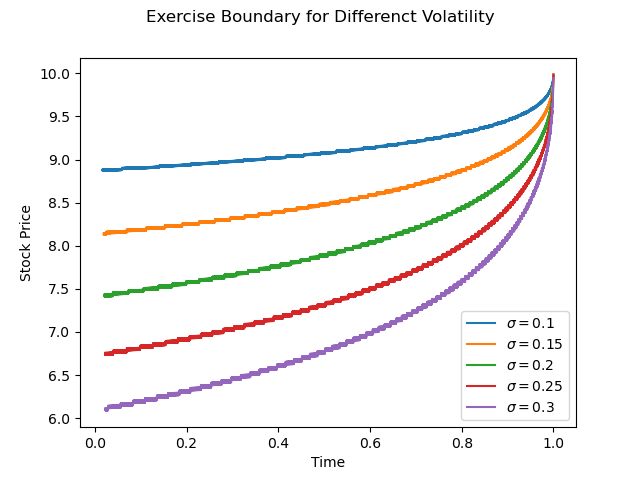
\includegraphics[width=\linewidth]{3a-iii-boundary-sigma.png}
  \end{subfigure}%
  \caption[]{Exercise Boundary with Different Risk-free Rate or Volatility}
\end{figure}

\subsection{Simulation}
Simulation analysis is the model that is applied to analyze a large database and determine the changes in input variables. The model uses simulations to predict how the outcome of a decision 
would vary in a given random situation. In the option simulation plot below, it displays a plot of 10000 simulated paths with different outcomes for the stock price, providing a wider sample 
space to emulate realistic scenarios.

\begin{figure}[H]
  \centering
  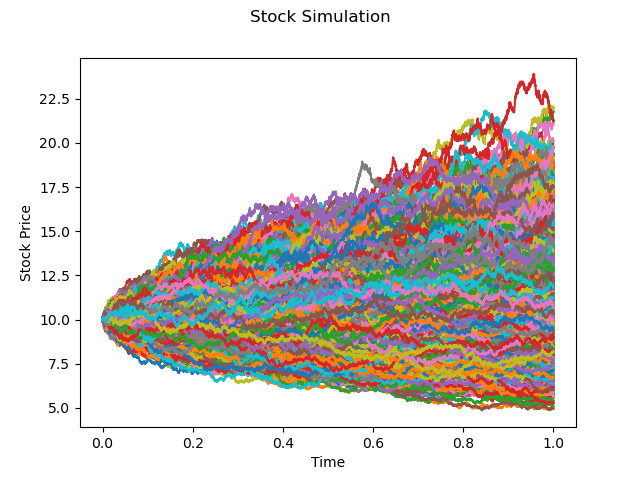
\includegraphics[scale=0.49]{3b-i-simulation.png}
  \caption[Asset Price Simulation]{Asset Price Simulation}
\end{figure}

\subsubsection{Profit \& Loss Analysis}
In this report, profit and loss of an option is defined as the present value of the payoff of the option at a specific time subtracting its price at inital time $t=0$. 
\\i.e.
\[\text{P\&L of option} = PV(\text{payoff of option}) - \text{option price}\]
According to the kernel density estimate of the P\&L model shown below, the plot is right-skewed where the mean is less than the median. Additionally, the peak of the plot appeared at the point when the 
P\&L is less than -0.5, indicating most simulated price paths do not hit the exercise boundary and get options exercised. Therefore, there is a net loss equaling the option price.
\begin{figure}[H]
  \centering
    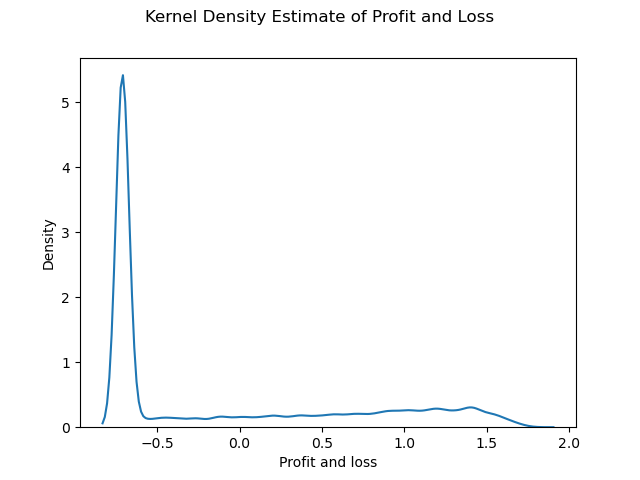
\includegraphics[scale=0.63]{3b-i-P&L.png}
    \caption[Kernel Density Estimate of P\&L]{Kernel Density Estimate of P\&L}
\end{figure}

\subsubsection{Exercise Time Analysis}
Time analysis is a way of analyzing a sequence of data points collected over an interval of time. The kernel density plot in this report is the main way to visualize the trend for time analysis.
\\\\
The kernel density estimate of time to maturity is left-skewed, where the mean is higher than the median. The peak of the plot appears at the point around $t=1$, indicating that long-term maturity 
time happens more frequently and gains more preferences in the market. And most simulated price paths do not hit the exercise boundary and get options exercised.
As the time closes to maturity, the density of exercise time becomes larger which indicates the option gains more preferences over time. 
Connecting with the research on risk above, the longer the maturity, greater risks may have an impact while along with the possible higher return as well, which best explains the trends of the plot.


\begin{figure}[H]
  \centering
    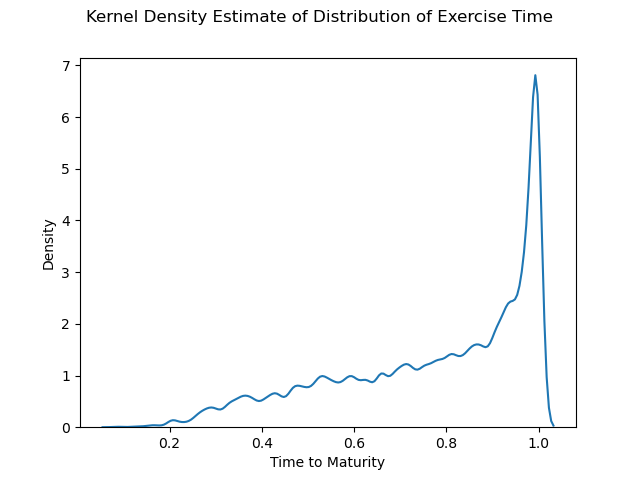
\includegraphics[scale=0.63]{3b-i-exercise_t.png}
    \caption[Kernel Density Estimate of Exercise Time]{Kernel Density Estimate of Exercise Time}
\end{figure}

\subsubsection{Sensitivity Analysis Ragarding Volatility}
By testing the volatility between 10\% and 30\% and the exercise boundary is build based on volatility $\sigma = 20\%$. The overall trends for the profit and loss plot are right-skewed, 
providing evidence that the mean is greater than the median for the simulated sample space. The overall trends for the exercise time plot are left-skewed, providing evidence that the median is greater 
than the mean for the simulated sample space.\\\\
The financial meanning behind these two opposite skewed graphs is that when volatility gets lower, the kernel density spike tends to be lower. 
That means as $\sigma$ increases, more simulated price paths do not hit the exercise boundary and get the put option exercised. A consequence of it is that these price paths end up having a net loss equaling 
the option price. This makes sense because as volatility increases, there are more chances for the simulated path to reach benchmark exercise boundary based on volatilty $\sigma=0.2$, hence more options corresponding to 
their price paths get exercised and even early exercised.

\begin{figure}[H]
  \centering
  \begin{subfigure}{.5\textwidth}
    \centering
    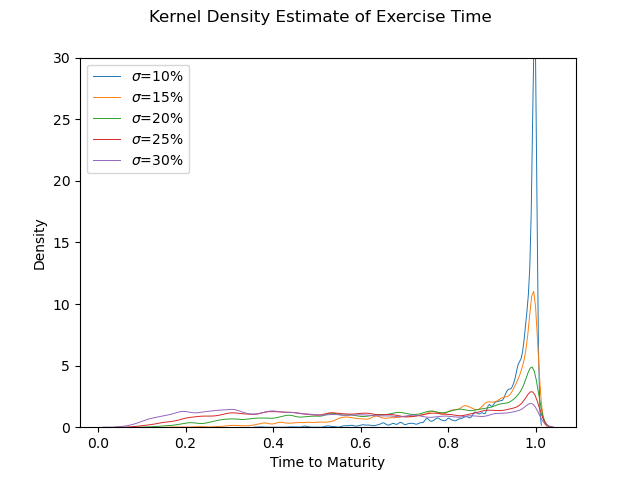
\includegraphics[width=\linewidth]{3b-ii-exercise_t.png}
  \end{subfigure}%
  \begin{subfigure}{.5\textwidth}
    \centering
    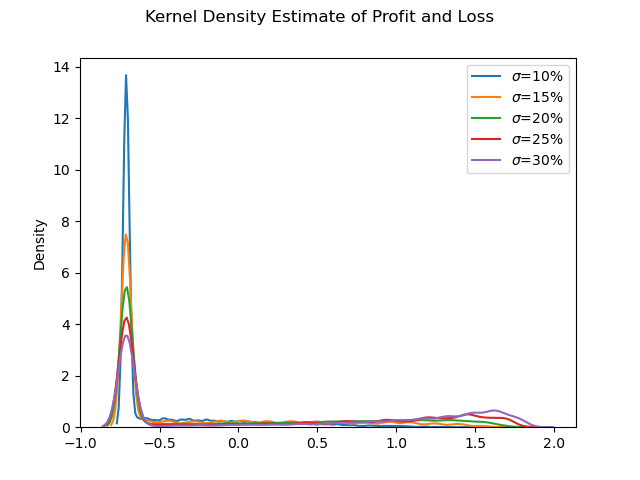
\includegraphics[width=\linewidth]{3b-ii-P&L.png}
  \end{subfigure}%
  \caption[]{Kernel Density Estimate of Exercise Time and P\&L with Various Realized Volatility}
\end{figure}

\section{Conclusion}
The report introduces the American put option from the perspective of the binomial tree and CRR model 
with slight adjustments. Starting with the algorithm and proof of the theories, and followed by the  
visualization of the model under the sample space and changes on parameters, the adjusted CRR model has shown 
the regulations of the American put options and how to evaluate their behaviors. The Sensitivity test discusses 
the effect of volatility and risk-free rate movements toward stock price and proves that risk goes high when 
volatility and risk-free rate increase. In the $\alpha$ and $\beta$ hedging strategies, the differences between the 
American options and European options are considered as the main factor that shows on the plot, and that helps 
explain the risk fluctuations between the two options. Lastly, the simulation test figures out the effect brought 
by various parameters on the distribution of profit \& loss according to the kernel density function. All the 
testing and simulations provided in the report create a complete view of understanding American put options.


\end{document}